\chapter{Documentazione driver per SCO-Board}
\label{appendiceA}
\thispagestyle{empty}
%% TODO App A: Leggere documentazione SCO-BOARD
\textit{Questa appendice contiene una breve descrizione dei driver sviluppati per interfacciare la SCO-Board con la scheda di sviluppo NI9636}

\section*{VI sviluppati}
Per consentire la comunicazione tra la scheda di conversione SCO-Board e la scheda di sviluppo NI9636 è stato necessario lo sviluppo di un apposito driver. Si è scelto di rendere disponibile una versione completa dei driver per consentire il riutilizzo della scheda di conversione per lavori futuri. 
Per la distribuzione si è scelto di fornire un archivio \textit{.zip} contenente i VI necessari scaricabile da \textit{github} \cite{sourceforge}.

I VI che fanno parte del set di driver sviluppato sono
\begin{itemize}
	\item Output enable-disable: abilita o disabilita i pin di uscita
	\item Clock pin init: abilita o disabilita i pin di clock
	\item Clock generator: genera il segnale di clock sincrono per DAC ed ADC
	\item Single point acquisition: acquisisce un campione dei dati in ingresso
	\item Single point generation: genera un campione di dati sulle uscite
\end{itemize}

Di seguito sarà descritta in dettaglio la struttura di ciascun VI e sarà spiegato in dettaglio come utilizzare il driver sviluppato all'interno di un software LabVIEW.
Per la descrizione di ingressi ed uscite si è scelto di utilizzare la convenzione di LabVIEW, segnando in grassetto gli ingressi necessari all'esecuzione del VI.

\subsection*{Output enable-disable}

\begin{figure}[H]
	\begin{center}
		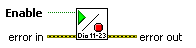
\includegraphics[scale=1]{appendiceA/enable_output}
		\caption{Struttura VI Output enable-disable}
	\end{center}
\end{figure}

Questo VI consente di abilitare e disabilitare i pin di uscita della scheda di sviluppo a cui si connette la SCO-Board, in modo da permettere il loro utilizzo per inviare un segnale digitale da 12-bit al convertitore presente sulla scheda di conversione.

\paragraph{Input}
\begin{itemize}
	\item \textbf{Enable:} consente di scegliere se abilitare o disabilitare le uscite digitali a cui è collegata la SCO-Board.
	\item Error in: consente di inserire in ingresso al VI un errore, per propagarlo nel codice o per ragioni di sincronizzazione.
\end{itemize}

\paragraph*{Output}
\begin{itemize}
	\item Error out: mostra se l'operazione è avvenuta con successo. In caso di errore mostra un codice di errore.
\end{itemize}

\subsection*{Clock pin init}

\begin{figure}[H]
	\begin{center}
		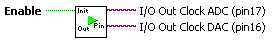
\includegraphics[scale=1]{appendiceA/clock_init}
		\caption{Struttura VI Clock pin init}
	\end{center}
\end{figure}

Questo VI consente di abilitare o disabilitare i pin che forniscono il clock ai convertitori della scheda di acquisizione SCO-Board.
\paragraph*{Input}
\begin{itemize}
	\item \textbf{Enable:} consente di scegliere se abilitare o disabilitare le uscite digitali a cui sono collegati i clock dei convertitori.
\end{itemize}

\paragraph*{Output}
\begin{itemize}
	\item I/O out clock ADC: indica il pin associato al clock dell'ADC.
	\item I/O out clock DAC: indica il pin associato al clock del DAC.
\end{itemize}

\subsection*{Clock generator}

\begin{figure}[H]
	\begin{center}
		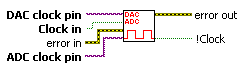
\includegraphics[scale=1]{appendiceA/clock_gen}
		\caption{Struttura VI Clock generator}
	\end{center}
\end{figure}

Questo VI si occupa di generare sulle uscite della scheda di sviluppo NI9636 il segnale logico all'ingresso del VI. Le uscite su cui questo segnale è generato sono associate ai clock del DAC e dell'ADC. Il VI genera il clock per i due convertitori in modo sincrono.

\paragraph*{Input}
\begin{itemize}
	\item \textbf{DAC clock pin:} pin associato al clock del DAC.
	\item \textbf{ADC clock pin:} pin associato al clock dell'ADC.
	\item \textbf{Clock in:} valore logico del clock da generare.
	\item Error in: consente di inserire in ingresso al VI un errore, per propagarlo nel codice o per ragioni di sincronizzazione.
\end{itemize}

\paragraph*{Output}
\begin{itemize}
	\item Error out: mostra se l'operazione è avvenuta con successo. In caso di errore mostra un codice di errore.
	\item !Clock: valore logico in ingresso negato.
\end{itemize}

\subsection*{Single point acquisition}

\begin{figure}[H]  
	\begin{center}
		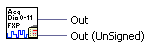
\includegraphics[scale=1]{appendiceA/acquisition}
		\caption{Struttura VI Single point acquisition}
	\end{center}
\end{figure}

Questo VI acquisisce un singolo campione in uscita dall'ADC. In accordo con le psecifiche fornite per l'ADC, l'acquisizione del dato sarà eseguita sul fronte di discesa del clock dell'ADC.
Il VI restituisce un valore numerico puro, espresso in \textit{fixed point da 12-bit, con parte intera da 12-bit}. Sono forniti sia il valore con segno che senza segno.

\paragraph*{Input}
Questo VI non ha input

\paragraph*{Output}
\begin{itemize}
	\item Out: il valore numerico in uscita dall'ADC, senza segno (0;+4095).
	\item Out (Unsigned): il valore in uscita dall'ADC, con segno (-2018;+2047).
\end{itemize}

\subsection*{Single point generation}

\begin{figure}[H]  
	\begin{center}
		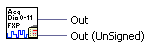
\includegraphics[scale=1]{appendiceA/acquisition}
		\caption{Struttura VI Single point acquisition}
	\end{center}
\end{figure}

Questo VI genera un singolo punto sulle uscite della scheda di sviluppo NI9636 associate agli ingressi del DAC. In accordo con le specifiche fornite per il DAC la generazione del dato sarà eseguita sul fronte di salita del clock del DAC. Il VI accetta in ingresso un valore numerico puro, espresso in \textit{fixed point da 12-bit, con parte intera da 12-bit, senza segno}.
\paragraph*{Input}
\begin{itemize}
	\item \textbf{Data to write:} il dato che si vuole generare espresso in fixed point senza segno (0;4095).
\end{itemize}

\paragraph*{Output}
\begin{itemize}
	\item Error out: mostra se l'operazione è avvenuta con successo. In caso di errore mostra un codice di errore.
\end{itemize}

\section*{Esempio di utilizzo del driver}
In questa sezione sarà mostrata la corretta procedura per implementare il driver SCO-Board all'interno di un applicativo LabVIEW.

Il progetto dell'applicativo LabVIW che farà uso del driver SCO-Board dovrà contenere tutti i VI contenuti nell'archivio \textit{.zip} fornito. La struttura delle cartelle dell'archivio non deve essere alterata.
Il progetto avrà la struttura mostrata in figura \ref{progetto}.

\begin{figure}[H]
	\begin{center}
		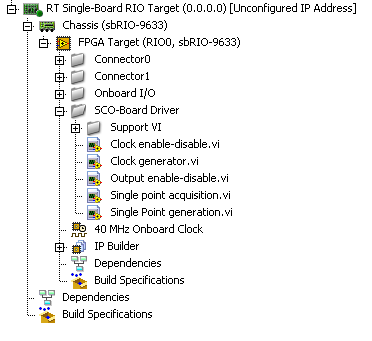
\includegraphics[scale=1]{appendiceA/progetto}
		\caption{Struttura del progetto contenente i driver SCO-Board}
		\label{progetto}
	\end{center}
\end{figure}

La struttura di un VI che fa uso dei driver SCO-Board è mostrata in figura \ref{VI}

\begin{figure}[H]
	\begin{center}
		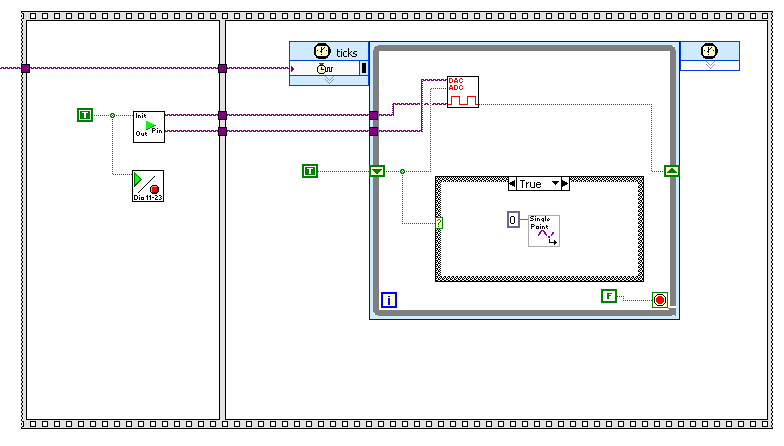
\includegraphics[scale=0.6]{appendiceA/VI}
		\caption{Struttura del VI contenente i driver SCO-Board}
		\label{VI}
	\end{center}
\end{figure}

Il VI sarà composto da una \textit{sequence structure}; il primo \textit{frame} della struttura avrà il compito di inizializzare le uscite della scheda di sviluppo NI9636, mentre il frame sucessivo conterrà il codice dell'applicazione.
All'intero del codice dell'applicazione è necessario inserire un \textit{single cycle timed loop}, con frequenza di clock doppia rispetto alla frequenza di campionamento, che conterrà il VI di generazione del clock e i VI di acquisizione e generazione del segnale. L'uso del \textit{single cycle timed loop} è necessario per garantire una temporizzazione precisa e coerente del clock.
All'intero del \textit{single cycle timed loop} sarà inserita una \textit{case structure} che garantirà la corretta sequenza e temporizzazione di acquisizione e generazione del segnale. In particolare la generazione sarà eseguita sel caso \textit{true} della \textit{case structure}, mentre l'acquisizione sarà eseguita nel caso \textit{false}.

Per lo scambio di dati con il resto dell'applicativo è consigliabile utilizzare il pattern producer-consumer.




